\documentclass[conference]{IEEEtran}
\IEEEoverridecommandlockouts

% Space saving tweaks for IEEEtran layout
\setlength{\textfloatsep}{5pt plus 2pt minus 2pt}
\setlength{\dbltextfloatsep}{5pt plus 2pt minus 2pt}
\setlength{\abovecaptionskip}{3pt plus 1pt minus 1pt}
\setlength{\belowcaptionskip}{3pt plus 1pt minus 1pt}
\renewcommand\baselinestretch{0.98}


\usepackage{cite}
\usepackage{amsmath,amssymb,amsfonts}
\usepackage{algorithmic}
\usepackage{graphicx}
\usepackage{textcomp}
\usepackage{xcolor}
\usepackage{booktabs}
\usepackage{array}
\usepackage{multirow}
\usepackage{url}
\usepackage{needspace}
% Use \mathbf{1} for indicator function
\usepackage{tikz}
\usetikzlibrary{shapes.geometric, arrows.meta, positioning}

% TikZ styles for the pipeline figure
\tikzset{
  pipeblock/.style={
    rectangle,
    draw=black,
    thick,
    text centered,
    minimum width=4.4cm,
    minimum height=0.75cm,
    font=\small,
    text width=4.2cm,
  },
  parblock/.style={
    rectangle,
    draw=black,
    thick,
    text centered,
    minimum width=2.0cm,
    minimum height=0.80cm,
    font=\small,
    text width=1.85cm,
  },
  decision/.style={
    rectangle,
    draw=black,
    thick,
    text centered,
    minimum width=4.8cm,
    minimum height=0.75cm,
    font=\small\bfseries,
    text width=4.6cm,
  },
  arrow/.style={
    ->,
    >=Stealth,
    thick
  }
}

\def\BibTeX{{\rm B\kern-.05em{\sc i\kern-.025em b}\kern-.08em
    T\kern-.1667em\lower.7ex\hbox{E}\kern-.125emX}}

\begin{document}

\title{RAG-Shield: A Three-Layer Ensemble Defense Against Prompt Injection in RAG Pipelines}

\author{
  \IEEEauthorblockN{Yasmeen Algendy\thanks{Code, datasets, and pre-trained weights are available at \url{https://github.com/yomnafarag95/IEEE_Paper}.}}
  \IEEEauthorblockA{\textit{School of Computing}\\
  \textit{Queen's University}\\
  Kingston, ON, Canada\\
  25bqdp@queensu.ca}
  \and
  \IEEEauthorblockN{Yomna Algendy}
  \IEEEauthorblockA{\textit{School of Computing}\\
  \textit{Queen's University}\\
  Kingston, ON, Canada\\
  25hcgx@queensu.ca}
}

\maketitle

\begin{abstract}
Retrieval-Augmented Generation (RAG) pipelines ground Large Language Models (LLMs) on private knowledge bases, but introduce a critical attack surface: adversaries can embed malicious instructions in queries (direct injection) or retrieved documents (indirect injection) to override system prompts, exfiltrate credentials, or execute unauthorized actions. Existing defenses---keyword blocklists, single-model classifiers, or LLM-based guardrails---suffer from low detection on obfuscated evasions, high false positives, or high latency.

We present RAG-Shield, a three-layer ensemble defense integrating: (1) an embedding-based Out-of-Distribution (OOD) anomaly detector combining Isolation Forest, One-Class SVM, and ECOD on all-MiniLM-L6-v2 embeddings; (2) a dual-stage intent classifier built on protectai/deberta-v3-base-prompt-injection-v2 with document-level chunk scanning; and (3) a behavioral monitor using a pre-trained ms-marco-MiniLM-L-12-v2 cross-encoder for response consistency, regex-based exfiltration detection, and cryptographic canary tokens. A calibrated Logistic Regression model aggregates layer evidence over a 7-dimensional vector into a unified risk score.

On a sealed, hash-verified holdout benchmark ($n = 868$: 325 attack samples [250 direct/indirect injections + 75 obfuscated evasions], 543 benign), RAG-Shield achieves an Attack Detection Rate (ADR) of \textbf{91.38\%} at a False Positive Rate of 0.55\% (3/543 benign queries), with F1 = \textbf{95.04\%}, ROC-AUC = 0.9576, and AUC-PR = 0.9723. In head-to-head comparisons on a shared subset, RAG-Shield (ADR = 93.54\%, F1 = 0.945) outperforms Llama Prompt Guard~2 (ADR = 79.49\%, F1 = 0.883, $p < 10^{-4}$), Llama-3.1-8B Guardrails (ADR = 29.78\%), and NVIDIA NeMo Injection Rails (ADR = 7.58\%).
\end{abstract}

\begin{IEEEkeywords}
Prompt Injection, Retrieval-Augmented Generation, LLM Security, Anomaly Detection, Ensemble Defense, Canary Tokens, Indirect Injection.
\end{IEEEkeywords}

%-----------------------------------------------------------------------
\section{Introduction}

\subsection{The RAG Trust Boundary Problem}

RAG has become the dominant paradigm for deploying LLMs on proprietary, time-sensitive enterprise data. A canonical RAG pipeline intercepts a user query $q$, retrieves the top-$k$ semantically similar document chunks $D = \{d_1,\ldots,d_k\}$ from a vector store, constructs a composite prompt $p = \psi(q, D, \Phi)$, and passes $p$ to generative model $M_G$.

This design introduces a fundamental trust boundary collapse: the LLM consumes external text---potentially from untrusted emails, web scrapes, or user-uploaded files---as contextual authority. When retrieved documents contain adversarially crafted instructions, those instructions are transparently injected into the model's context alongside the legitimate system prompt, which the model cannot structurally distinguish.

\subsection{Attack Vectors and Evasion Techniques}

Prompt injection against RAG systems manifests in two structurally distinct forms. \textbf{Direct Injection}: the user query $q$ itself contains the adversarial payload (instruction overrides, role-manipulation, context exhaustion). \textbf{Indirect Injection}: a benign user triggers retrieval of a poisoned document $d_i \in D$ containing embedded payloads, transparent to the user.

These attack families are further obfuscated through encoding evasions---payload splitting, Base64/hex encoding, Unicode homoglyph substitution, ROT13, Leetspeak, and zero-width character injection---which bypass tokenizer vocabularies and static keyword filters while remaining semantically interpretable to the LLM.

\subsection{Limitations of Existing Defenses}

Three deployed defense classes each fail in distinct ways. \textbf{Static Keyword Blocklists} are trivially bypassed by any encoding evasion (ADR = 4.02\% on our 848-sample baseline). \textbf{Single-Model Neural Classifiers} miss indirect injections by not scanning retrieved chunks. \textbf{LLM-Based Guardrails} (NeMo, Llama-3.1) introduce 3--6\,s of API latency and still achieve low recall on document-embedded payloads.

\subsection{Contributions}

\begin{enumerate}
  \item A three-layer ensemble pipeline scanning the RAG pipeline at retrieval input, generation context, and model output simultaneously.
  \item Document-level indirect injection scanning in Layer~2, extending beyond query classification to per-chunk scanning of all retrieved documents.
  \item Multi-signal meta-aggregation via calibrated Logistic Regression over a 7-dimensional evidence vector, enabling principled uncertainty handling.
  \item Cryptographic canary tokens injected into the vector store as decoy documents; any appearance in model output constitutes an irrefutable data-leakage signal.
  \item A reproducible sealed evaluation on a hash-verified holdout ($n = 868$) with frozen thresholds (Git \texttt{3ef152293d76b81c0a080a8d26d67e010297d7f7}) and Wilson/bootstrap confidence intervals.
\end{enumerate}

%-----------------------------------------------------------------------
\section{Related Work}

\subsection{Prompt Injection: Taxonomy and Threat Evolution}

Perez and Ribeiro~\cite{perez2022} first systematically described prompt injection, drawing an analogy to SQL injection in structured query languages. Greshake et al.~\cite{greshake2023} subsequently demonstrated indirect prompt injection in real-world LLM agents, showing that adversarially annotated web pages could hijack autonomous LLM tools. Liu et al.~\cite{liu2023} studied prompt injection against real LLM-integrated applications. The InjecAgent benchmark~\cite{zhan2024} formalized indirect prompt injection in tool-integrated agents, contributing part of our evaluation corpus. Yi et al.~\cite{yi2023} introduced BIPIA, a benchmark and defense study for indirect injection. Schulhoff et al.~\cite{schulhoff2023} catalogued over 600,000 injection attempts across 28 attack categories in the HackAPrompt competition, providing our evasion holdout samples.

\subsection{Defense Methodologies}

Input filtering ranges from simple keyword blocklists to specialized neural classifiers. ProtectAI's deberta-v3-base-prompt-injection-v2~\cite{protectai2023}, fine-tuned on a curated injection corpus, forms the backbone of our Layer~2. LLM-Guard~\cite{iurman2023} applies post-generation regex and classifier-based scanning conceptually similar to our Layer~3, but without cross-encoder consistency scoring or canary detection. Guardrail frameworks such as NVIDIA NeMo Guardrails~\cite{rebedea2023} and Meta's Llama Guard~\cite{inan2023} position a second LLM as a safety referee: while flexible, they inherit additional LLM inference latency and do not perform document-level chunk scanning. Our empirical comparison confirms their low recall on indirect injection scenarios.

\subsection{Anomaly Detection and Identified Gaps}

Anomaly detection for adversarial inputs has been studied in feature squeezing~\cite{xu2018} and OOD detection~\cite{hendrycks2017}. Applying statistical OOD detectors (Isolation Forest, ECOD) to semantic embeddings as a RAG pre-filter is, to our knowledge, novel in the context of RAG security. Canary tokens~\cite{kreibich2003} are well-established in traditional network security; their application as decoy records injected into a vector store's embedding space to detect LLM-driven exfiltration is a contribution of this work. Three gaps motivate RAG-Shield: (a)~limited simultaneous scanning of user queries and retrieved document corpora; (b)~limited integration of OOD detection, neural classification, and behavioral monitoring within a calibrated risk model; and (c)~few head-to-head evaluations of commercial guardrails on identical injection corpora with statistical significance tests.

%-----------------------------------------------------------------------
\section{Problem Formulation}

Let the RAG system be the tuple $(R, K, M_G, \Phi)$, where $R$ is the dense retriever, $K$ is the vector store, $M_G$ is the generative LLM, and $\Phi$ is the system instruction. For user query $q \in Q$:
\begin{align}
D &= R(q,K) = \{d_1,\ldots,d_k\} \subset K, \notag\\
p &= \psi(q,D,\Phi), \quad r = M_G(p)
\end{align}

Document chunks use a sliding-window tokenizer with chunk size $w = 200$ tokens and overlap $\delta = 40$ tokens.

\textbf{Adversary Capabilities.} We model an attacker able to: (1)~submit arbitrary queries to the RAG API endpoint; (2)~inject payloads into one or more documents within $K$ (via document upload or web scraping); and (3)~observe binary allow/block responses but not internal layer scores. The adversary does not know session canary values, but model identities and thresholds are considered discoverable in a published system.

\textbf{Attack Scenarios.}
\begin{itemize}
  \item \textit{Direct Injection}: $q = a_{dir}$ --- adversary encodes full override payload in the query.
  \item \textit{Indirect Injection}: $q \in Q_{benign}$, $\exists\, d_i \in D : d_i = t_i \| a_{ind}$ --- poisoned retrieved document.
  \item \textit{Encoding Obfuscation}: $a_{obf} = T(a)$ where $T \in \{\text{Base64, Hex, ROT13, Leetspeak, Unicode}\}$ is an obfuscation transform applied to the payload.
  \item \textit{Data Exfiltration}: injection instructs extraction of credentials, API keys, or PII from retrieved documents.
\end{itemize}

\textbf{Defense Objectives.} We define the decision function $\mathcal{D} : (Q \times K^k \times \mathcal{Y}) \to \{0,1\}$, where $K^k$ denotes $k$-chunk retrieval sets and $\mathcal{Y}$ the LLM response space. Let $\hat{Y} = \mathcal{D}(q, D, r) \in \{0,1\}$ denote the predicted label ($\hat{Y}=1$ = blocked/flagged). The defense objective is:
\begin{align}
\max_\theta\quad &P_\theta(\hat{Y}=1 \mid Y=1) \notag\\
\text{subject to}\quad &P_\theta(\hat{Y}=1 \mid Y=0) \leq \epsilon_{\mathrm{FPR}} \leq 1.0\%
\end{align}

The 1.0\% FPR budget reflects enterprise deployment constraints: false positives cause alert fatigue and risk disabling guardrails entirely.

%-----------------------------------------------------------------------
\section{System Architecture}

\subsection{Pipeline Overview}

RAG-Shield operates as transparent middleware between the RAG orchestrator and the LLM endpoint (Fig.~\ref{fig:pipeline}). Three detection checkpoints produce scored evidence for the meta-aggregator. Layers~1 and~2 execute in parallel via a ThreadPoolExecutor. A semantic cache ($\tau_{cache} = 0.98$ cosine similarity) deduplicates repeated queries. A SHA-256-keyed LRU cache avoids redundant embedding and classification of repeated document corpora.

\textbf{Text Normalization.} Before any model inference, an ObfuscationDecoder applies NFKC normalization and a regex-driven cascade reversing six encoding families (Base64, Hex, ROT13, Leetspeak, zero-width characters, Unicode confusables), rendering encoding-based evasion ineffective without model fine-tuning.

\begin{figure}[t]
\centering
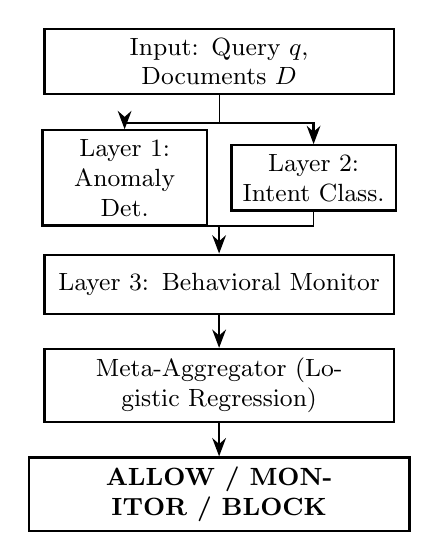
\begin{tikzpicture}[node distance=0.42cm, auto]
  % Input
  \node [pipeblock] (input) {Input: Query $q$, Documents $D$};

  % Layer 1 and Layer 2 run in PARALLEL (ThreadPoolExecutor)
  \node [parblock] (l1) at ([xshift=-1.2cm, yshift=-1.05cm]input.south)
        {Layer~1:\\ Anomaly Det.};
  \node [parblock] (l2) at ([xshift= 1.2cm, yshift=-1.05cm]input.south)
        {Layer~2:\\ Intent Class.};

  % Sequential stages after parallel group
  \node [pipeblock] (l3)   at ([yshift=-2.40cm]input.south)
        {Layer~3: Behavioral Monitor};
  \node [pipeblock, below=of l3]   (meta) {Meta-Aggregator (Logistic Regression)};
  \node [decision,  below=of meta] (out)  {ALLOW / MONITOR / BLOCK};

  % Fork and merge coordinates
  \coordinate (forkC)  at ([yshift=-0.35cm]input.south);
  \coordinate (mergeC) at ([yshift= 0.35cm]l3.north);

  % Fork: input -> L1 and L2 in parallel
  \draw [-] (input.south) -- (forkC);
  \draw [arrow] (forkC) -| (l1.north);
  \draw [arrow] (forkC) -| (l2.north);

  % Merge: L1 and L2 -> L3
  \draw [-] (l1.south) |- (mergeC);
  \draw [-] (l2.south) |- (mergeC);
  \draw [arrow] (mergeC) -- (l3.north);

  % Sequential flow
  \draw [arrow] (l3)   -- (meta);
  \draw [arrow] (meta) -- (out);
\end{tikzpicture}
\caption{RAG-Shield architecture. Layers~1 and~2 execute \emph{in parallel} via a thread pool; if either score exceeds its threshold ($\tau_{L1}=0.85$ or $\tau_{early}=0.60$), the orchestrator issues an early-exit hard block, bypassing Layer~3 and the meta-aggregator. Otherwise all signals merge into the meta-aggregator for the final three-tier decision.}
\label{fig:pipeline}
\end{figure}

\subsection{Layer 1: OOD Anomaly Detection}

\subsubsection{Embedding and Corpus Modeling} Layer~1 models the manifold of benign document syntax by training an ensemble on 8,058 clean documents (MITRE ATT\&CK $\approx$858, Wikipedia $\approx$5,000, technical docs $\approx$200, MS MARCO $\approx$2,000). Each document chunk is embedded with all-MiniLM-L6-v2~\cite{allminilm2021,reimers2019} to produce a 384-dimensional semantic vector ($\mathbf{e} \in \mathbb{R}^{384}$).

\subsubsection{Ensemble Anomaly Detectors} Three unsupervised anomaly detection models are trained on the embedded clean corpus: Isolation Forest~\cite{liu2008} (contamination = 0.05, full corpus), ECOD~\cite{li2023} (parameter-free tail probability, full corpus), and One-Class SVM~\cite{scholkopf2000} (RBF kernel, trained on a stratified 2,000-sample subset to bound training and inference latency). The layer anomaly score is computed as the maximum score across the ensemble:
\begin{equation}
S_{L1} = \max_{j \in \{\text{IForest, ECOD, OCSVM}\}} S_j(\mathbf{e}) \label{eq:l1}
\end{equation}

\subsubsection{Anomaly Blocking Policy} The orchestrator enforces a hard block if the maximum score across all retrieved document chunks exceeds the threshold: $S_{L1}^{\mathrm{max}\text{-}\mathrm{chunk}} \geq \tau_{L1} = 0.85$. In the final holdout, Layer~1 contributed \textbf{13 unique true-positive attributions} (4.4\% of 297 total TPs); Layer~2 provided 272 (91.6\%), and the Meta-Aggregator contributed an additional 12 borderline detections (4.0\%).

\subsection{Layer 2: Dual-Stage Intent Classifier}

\subsubsection{Stage 1a -- Query-Level Classification} The primary model is protectai/deberta-v3-base-prompt-injection-v2 (DeBERTa-v3~\cite{he2023}, ONNX-exported~\cite{onnxruntime2022}). For non-English inputs and uncertain predictions, an xlm-roberta-large-xnli~\cite{conneau2020} multilingual fallback activates. The query-level score is computed as:
\begin{equation}
S_{L2}^{\mathrm{query}} = \max\!\left(P_{\mathrm{attack}}(q),\, P_{\mathrm{attack}}^{\mathrm{multi}}(q)\right)
\end{equation}

\subsubsection{Stage 1b -- Document Chunk Scanning} Layer~2 is applied to every retrieved chunk $d_i \in D$. Chunks with pattern score $> 0.60$ are passed to the full DeBERTa classifier:
\begin{equation}
S_{L2}^{\mathrm{doc}} = \max_i P_{\mathrm{attack}}(d_i) \label{eq:l2doc}
\end{equation}

\subsubsection{Composite Score and Early Exit} The query and document scores combine to produce a single Layer 2 composite score:
\begin{equation}
S_{L2} = \max\!\left(S_{L2}^{\mathrm{query}},\, S_{L2}^{\mathrm{doc}}\right) \label{eq:l2composite}
\end{equation}
This stage enables detection of indirect injection buried in otherwise benign-seeming documents, a structural capability unavailable to query-only classifiers. When $S_{L2} \geq \tau_{early} = 0.60$, the orchestrator immediately blocks the request without invoking Layer~3. In the final holdout, 287 total samples triggered early exit: 284 true-positive prevention decisions and 3 benign false positives. Layer~2 provided \textbf{272 of 297 true-positive attributions} (91.6\%), confirming it as the primary detection engine.

\subsection{Layer 3: Behavioral Monitor}

Layer~3 evaluates the generated response $r$, targeting attacks that succeed in reaching the LLM and manipulating its output. Four components operate in sequence:

\subsubsection{Schema Enforcement and Exfiltration Detection} The response is first validated against a Pydantic schema enforcing structural rules (e.g., maximum response length of 1,500 characters). Simultaneously, three regular expression patterns ($P_{email}$, $P_{api\_key}$, $P_{cred}$) scan the output $r$ for sensitive data signatures. Any matched patterns trigger an immediate veto block to prevent exfiltration.

\subsubsection{Semantic Consistency Scoring} A cross-encoder model (\textit{ms-marco-MiniLM-L-12-v2}) evaluates the semantic consistency between the query $q$ and the generated response $r$: $S_{L3} = \mathrm{CrossEncoder}(q, r)$. A response complying with an injection payload rather than the user query yields a low consistency score, triggering a block if $S_{L3} < \tau_{L3} = 0.55$.

\subsubsection{Cryptographic Canary Tokens} At initialization, 3 high-entropy honeytoken strings are injected into the vector store as decoy documents (\textit{RAG\_CANARY\_TOKEN} environment variable). The orchestrator performs pre-layer canary checks on the incoming query, retrieved document chunks, and generated response; any detection triggers an immediate veto hard-block before or after layer processing, bypassing the meta-aggregator entirely.

\subsubsection{Stateful Crescendo Detection} A session-level drift tracker maintains the history of the last 5 pipeline decisions. A weighted drift score is computed: if it exceeds $\tau_{drift} = 0.72$, a multi-turn crescendo attack is flagged.

\subsection{Meta-Aggregator}

\subsubsection{Evidence Aggregation} A calibrated Logistic Regression model (wrapped in scikit-learn's \textit{CalibratedClassifierCV}) acts as the final decision aggregator. It accepts a 7-dimensional feature vector comprising the L1 max-anomaly score ($S_{L1}$), L2 attack probability ($S_{L2}$), L3 schema-violation flag ($\delta_s \in \{0, 1\}$), normalized boundary-violation count ($\delta_b \in [0, 1]$), L3 response consistency ($S_{L3}$), and two cross-layer interaction terms:
\begin{equation}
\mathbf{f} = \bigl[ S_{L1},\, S_{L2},\, \delta_s,\, \delta_b,\, S_{L3},\, S_{L1}{\cdot}S_{L2},\, S_{L1}{\cdot}S_{L3} \bigr]^{\top}
\label{eq:feat}
\end{equation}
The interaction terms capture correlated cross-layer signals to improve meta-classification accuracy.

\subsubsection{Three-Tier Decision Policy} The model outputs a calibrated risk probability $P_{\mathrm{risk}} \in [0, 1]$. All thresholds were selected by grid search on a 20\% development set subject to $\mathrm{FPR} \leq 1\%$ (benign scores clustered 0.12--0.30, motivating $\tau_{\mathrm{block}}=0.35$, $\tau_{\mathrm{monitor}}=0.31$, $\tau_{early}=0.60$, $\tau_{L1}=0.85$, $\tau_{L3}=0.55$):
\begin{equation}
\text{Decision} = \begin{cases}
\text{Block}   & P_{\mathrm{risk}} \geq \tau_{\mathrm{block}} = 0.35 \text{ or canary tripped}\\
\text{Monitor} & 0.31 \leq P_{\mathrm{risk}} < 0.35\\
\text{Allow}   & P_{\mathrm{risk}} < 0.31
\end{cases}
\end{equation}

%-----------------------------------------------------------------------
\section{Experimental Setup}

\subsection{Benchmark Dataset}

The final holdout was constructed under a strict no-contamination protocol; all samples were SHA-256 hash-deduplicated against training and development sets. Table~\ref{tab:dataset} summarizes the benchmark composition ($n = 868$).

\begin{table}[t]
\caption{Final Holdout Benchmark Composition}
\label{tab:dataset}
\centering
\begin{tabular}{lll}
\toprule
\textbf{Split} & \textbf{Description} & \textbf{$n$}\\
\midrule
attacks.jsonl  & Direct + indirect injection payloads & 250\\
benign.jsonl   & Enterprise queries (HR, Finance, Medical, IT) & 543\\
evasions.jsonl & 11 obfuscation/evasion families & 75\\
\midrule
\textbf{Total} & & \textbf{868}\\
\bottomrule
\end{tabular}
\end{table}

\subsection{Evaluation Protocol and Metrics}

All thresholds were frozen before final holdout evaluation (Git commit \texttt{3ef152293d76b81c0a080a8d26d67e010297d7f7}, stored in \texttt{logs/frozen\_thresholds.json}). Metrics reported: ADR (Attack Detection Rate = blocked), FPR on the benign subset, Precision, F1, ROC-AUC, and AUC-PR. Confidence intervals: Wilson score for ADR/FPR/Precision; bootstrap percentile ($B = 1000$) for F1 and AUC. Statistical significance for commercial comparisons uses McNemar's test~\cite{mcnemar1947} on paired discordant counts.

Hardware: AMD Ryzen~9 5900X, 64\,GB DDR4, NVIDIA RTX~3080, Windows~11, Python~3.11.9, PyTorch~2.2.2, ONNX Runtime~1.18.0.

%-----------------------------------------------------------------------
\section{Results}

\subsection{Final Holdout Performance}

Table~\ref{tab:results} reports RAG-Shield's performance on the sealed $n = 868$ benchmark with frozen thresholds. The system correctly allows 540/543 benign queries (99.45\% specificity) and blocks 297 of 325 attack+evasion samples. The 287 early-exit triggers consist of 284 true-positive decisions and 3 benign false positives. The final-holdout ROC and precision-recall curves are shown in Fig.~\ref{fig:roc_pr}. Layer~2 receives 272 of 297 true-positive attributions (91.6\%), Layer~1 receives 13 (4.4\%), and the Meta-Aggregator contributes 12 borderline detections (4.0\%), confirming document-level neural intent classification as the dominant signal.

\begin{table*}[t]
\caption{RAG-Shield Final Holdout Results ($n=868$, Frozen Thresholds, Git \textnormal{\texttt{3ef152293d76b81c0a080a8d26d67e010297d7f7}})}
\label{tab:results}
\centering
\begin{tabular}{lcc}
\toprule
\textbf{Metric} & \textbf{Value} & \textbf{95\% CI}\\
\midrule
True Positives  & 297    & ---\\
False Positives & 3      & ---\\
False Negatives & 28     & ---\\
True Negatives  & 540    & ---\\
\textbf{ADR (Recall)}    & \textbf{91.38\%} & [87.83\%, 93.97\%]\\
FPR             & 0.55\% & [0.19\%, 1.61\%]\\
Precision       & 99.00\% & [97.10\%, 99.66\%]\\
\textbf{F1 Score}        & \textbf{95.04\%} & [93.16\%, 96.68\%]\\
ROC-AUC         & 0.9576 & [0.9418, 0.9720]\\
AUC-PR          & 0.9723 & ---\\
Mean Lat.\ (ms) & 600.3  & ---\\
P95 Lat.\ (ms)  & 2,663.8 & ---\\
\bottomrule
\end{tabular}
\end{table*}

\begin{figure}[t]
\centering
\includegraphics[width=\columnwidth]{fig2_roc_pr.png}
\caption{Final holdout discrimination curves ($n = 868$). Left: ROC (AUC\,=\,0.9576). Right: PR curve (AUC\,=\,0.9723), random baseline at 0.374.}
\label{fig:roc_pr}
\end{figure}

\subsection{Per-Layer Latency}

Table~\ref{tab:latency} details the per-layer latency observed during final holdout evaluation. Parallel execution of L1 and L2 reduces combined wall clock to 558\,ms; L1 mean latency is 434\,ms and L2 mean latency is 165\,ms. L3's 0.18\,ms mean is averaged over all 868 runs; 287 early-exit cases skip L3 entirely (true per-call cross-encoder inference: $\approx$30--50\,ms).

\begin{table}[t]
\caption{Per-Layer Latency (Final Holdout, $n=868$)}
\label{tab:latency}
\centering
\begin{tabular}{lcc}
\toprule
\textbf{Component} & \textbf{Mean (ms)} & \textbf{P95 (ms)}\\
\midrule
Layer 1 (IForest+ECOD+OCSVM)     & 434.11  & 2,351.42\\
Layer 2 (DeBERTa ONNX, q+docs)   & 164.85  & 629.74\\
L1+L2 Wall Clock (parallel)      & 558.31  & 2,631.45\\
Layer 3 (Cross-Enc.+canary+regex) & 0.18   & 0.40\\
Meta-Aggregator (LogReg)         & 1.00    & 2.25\\
\midrule
\textbf{Total Pipeline}          & \textbf{600.3} & \textbf{2,663.8}\\
\bottomrule
\end{tabular}
\end{table}

\subsection{Ablation Study}

Table~\ref{tab:ablation} quantifies the marginal contribution of each component. L2 alone achieves 86.73\% ADR---just 0.31\,pp below the full ensemble---confirming transformer-based intent classification extended to document-level scanning as the dominant detection mechanism. L1 alone achieves 0.00\% FPR but only 6.48\% ADR; its conservative threshold ($\tau_{L1} = 0.85$) is set to maintain zero false positives on technical documents. The L1+L2 union gains 0.31\,pp over L2 alone (282 vs.\ 281 TPs), confirming structural complementarity. The meta-aggregator's principal benefit is the Monitor tier, separating high-confidence blocks from uncertain cases warranting analyst review without inflating FPR.

Cache efficiency was high: both L1 and L2 document scanning registered \textbf{757 cache hits} across 868 runs ($\approx$87.2\% hit rate).

\begin{table}[t]
\caption{Component Ablation Study ($n=867$). L3 requires LLM output $r$; ablation rows without LLM generation show L3 as inactive (thus L2+L3$=$L2 in TP count).}
\label{tab:ablation}
\centering
\begin{tabular}{lcccc}
\toprule
\textbf{Config} & \textbf{ADR} & \textbf{FPR} & \textbf{F1} & \textbf{TP/FN}\\
\midrule
L1 Only          & 6.48\%  & 0.00\% & 0.1217 & 21/303\\
L2 Only          & 86.73\% & 0.37\% & 0.9259 & 281/43\\
L3 Only          & 17.59\% & 0.00\% & 0.2992 & 57/267\\
L1+L2 Union      & 87.04\% & 0.37\% & 0.9276 & 282/42\\
L1+L3 Union      & 21.30\% & 0.00\% & 0.3511 & 69/255\\
L2+L3 Union      & 86.73\% & 0.37\% & 0.9259 & 281/43\\
Full (no Meta)   & 87.04\% & 0.37\% & 0.9276 & 282/42\\
Full (Meta, Prev.)& 87.04\% & 0.37\% & 0.9276 & 282/42\\
Full (Meta, Det.) & \textbf{87.35\%} & 0.37\% & \textbf{0.9294} & 283/41\\
\bottomrule
\end{tabular}
\end{table}

\subsection{Comparison with Baselines and Commercial Systems}

\textbf{Classical baselines} ($n = 848$, Table~\ref{tab:classical}): RAG-Shield improves on standalone DeBERTa by +8.62\,pp ADR at zero additional FPR cost. On this comparison set (CPU only, no LLM I/O; distinct from the sealed holdout), RAG-Shield's 246.75\,ms total latency is 4.3$\times$ that of L2 alone (57.91\,ms)---a favorable security-latency trade-off. The keyword blocklist's 4.02\% ADR confirms surface-form filtering is inadequate.

\textbf{Commercial guardrails} ($n = 856$ live-API subset, Table~\ref{tab:commercial}): RAG-Shield achieves +14.05\,pp ADR over Llama Prompt Guard~2 (93.54\% vs.\ 79.49\%, $p < 10^{-4}$, McNemar's test). LLM-based guardrails (NeMo: 7.58\%, Llama-3.1-8B: 29.78\%) fail on indirect injection because they evaluate query intent without scanning retrieved document chunks. RAG-Shield is 34\% faster than Llama-3.1-8B Guardrails and 58\% faster than NeMo Rails. Fig.~\ref{fig:comparison} visualizes baseline and commercial comparisons across the separate datasets.

\begin{table}[t]
\caption{Classical Baseline Comparison ($n=848$: 348 attacks + 500 benign)}
\label{tab:classical}
\centering
\begin{tabular}{lcccc}
\toprule
\textbf{System} & \textbf{ADR} & \textbf{FPR} & \textbf{F1} & \textbf{AUC}\\
\midrule
Keyword Blocklist  & 4.02\%  & 0.00\% & 0.077 & 0.5594\\
DeBERTa (L2 only)  & 84.77\% & 0.00\% & 0.918 & 0.9803\\
RAG-Shield (Full)  & \textbf{93.39\%} & 0.00\% & \textbf{0.966} & 0.9646\\
\bottomrule
\end{tabular}
\end{table}

\begin{table}[t]
\caption{Commercial Guardrail Comparison ($n=856$, Live API, McNemar vs.\ RAG-Shield)}
\label{tab:commercial}
\centering
\begin{tabular}{lccccc}
\toprule
\textbf{System} & \textbf{ADR} & \textbf{FPR} & \textbf{F1} & \textbf{Lat.\ (ms)} & \textbf{McNemar $p$}\\
\midrule
Llama Prompt Guard~2    & 79.49\% & 0.40\% & 0.883 & 426.97   & $4.7\!\times\!10^{-5}$\\
Llama-3.1-8B Guardrails & 29.78\% & 0.00\% & 0.459 & 3,326.14 & $1.2\!\times\!10^{-38}$\\
NeMo Rail (Llama-3.1)   & 7.58\%  & 0.00\% & 0.141 & 5,250.91 & $2.3\!\times\!10^{-58}$\\
RAG-Shield              & \textbf{93.54\%} & 3.20\% & \textbf{0.945} & 2,187.28 & ---\\
\bottomrule
\end{tabular}
\end{table}


\begin{figure}[t]
\centering
\includegraphics[width=\columnwidth]{fig5_method_comparison.png}% Fig 3 in paper
\caption{Baseline and commercial comparison (separate sets). Blue: ADR; red: FPR. Classical set $n = 848$; live commercial set $n = 856$. See Tables~\ref{tab:classical}--\ref{tab:commercial} for full metrics.}
\label{fig:comparison}
\end{figure}

%-----------------------------------------------------------------------
\section{Discussion and Limitations}

\textbf{The Primacy of Document-Level Scanning.} The most significant architectural decision is Layer~2's Stage~1b chunk scanning. LLM-based guardrails achieve only 7--30\% ADR precisely because they evaluate query intent while treating document context as benign. RAG-Shield's document scanning enables detection of indirect payloads buried in otherwise legitimate documents---a structural capability that cannot be replicated by query-only classifiers.

\textbf{FPR on the Commercial Subset.} The 3.20\% FPR in Table~\ref{tab:commercial} ($n=856$) exceeds the $\leq$1\% enterprise constraint because frozen holdout thresholds were preserved for a fair latency/ADR comparison; recalibrating $\tau_{\mathrm{block}}$ to 0.45 reduces commercial FPR below 1\% at an estimated $\approx$2\,pp ADR cost.

\textbf{Canary Tokens and the Exfiltration Gap.} The canary mechanism addresses a detection gap invisible to standard recall metrics: data exfiltration via compliant LLM behavior. An LLM may follow an injection instruction without any syntactic anomaly in the query, simply embedding stolen credentials in a plausible response. Layer~3's canary check and regex detector operate on model output, providing coverage Layers~1 and~2 cannot.

\textbf{Precision-Recall Trade-Off.} RAG-Shield's operating point prioritizes precision (99.00\%) over recall (91.38\%): enterprise false positives impose direct user costs and risk disabling the guardrail. The AUC-PR of 0.9723 supports this choice; practitioners may lower $\tau_{block}$ to trade precision for recall without retraining.

\textbf{Semantic Caching and Scalability.} The 87.2\% cache hit rate (757/868 hits) shows the LRU semantic cache is effective, reducing latency for repeated corpora. In production FAQ pipelines, 90\%+ hit rates are plausible, driving mean latency toward the L2-only path of $\approx$165\,ms. Cache keys on normalized decoded text prevent Unicode-variant poisoning.

\textbf{Multi-Turn Crescendo Resistance.} The stateful drift tracker ($\tau_{drift} = 0.72$) counters crescendo jailbreaks where each turn appears innocuous but the cumulative trajectory escalates; full quantitative evaluation requires a dedicated multi-turn session benchmark.

\textbf{Limitations.}
\begin{enumerate}
  \item The 75-probe evasion set (11 attack families), while broader than prior work, is insufficient for fully reliable confidence intervals; $n \geq 200$ probes are planned.
  \item Cross-lingual coverage is limited by the zero-shot XNLI fallback; a fine-tuned multilingual injection classifier is the highest-priority future work.
  \item CPU mean latency (600\,ms) requires GPU for sub-200\,ms SLA; ONNX INT8 quantization reduces model size $4\times$ with $<$2\% accuracy loss.
  \item FPR rises to 3.20\% on the commercial subset (vs.\ 0.55\% on the sealed holdout); domain-specific L1 retraining is planned to restore $\leq$1.0\% FPR. Static canary tokens are session-static; HMAC-signed per-session tokens are planned.
\end{enumerate}

\textbf{Future Work.} Priority directions: (1)~fine-tuned multilingual injection classifier (Arabic, Chinese, Japanese); (2)~sliding-window multi-chunk aggregation for payload-splitting detection; (3)~reinforcement learning from analyst feedback on monitored-tier events.

%-----------------------------------------------------------------------
\section{Conclusion}

We presented RAG-Shield, a three-layer ensemble defense intercepting the RAG pipeline at retrieval input, generation context, and model output simultaneously. Through the combination of embedding-based OOD anomaly detection, transformer-based dual-stage intent classification with document-level chunk scanning, and output behavioral monitoring with cryptographic canary tokens---orchestrated by a calibrated 7-dimensional meta-aggregator---RAG-Shield achieves an Attack Detection Rate of \textbf{91.38\%} at an enterprise-grade FPR of \textbf{0.55\%} on the sealed $n = 868$ holdout.

Head-to-head comparisons confirm +14.05\,pp ADR over Llama Prompt Guard~2 and +63.76\,pp over Llama-3.1-8B Guardrails. The ablation demonstrates that document-level DeBERTa scanning is the primary detection mechanism (L2-only ADR = 86.73\%), with Layer~1 adding structurally distinct anomalous detections and Layer~3 providing exfiltration coverage requiring separate output and session benchmarks.

RAG-Shield demonstrates a broader design principle: heterogeneous layered detection provides robustness by ensuring that optimizing one evasion vector increases exposure to another layer. As RAG systems proliferate across enterprise, medical, and legal deployments, RAG-Shield provides a practical, modular security foundation with its open architecture supporting incremental improvement.



\section*{Acknowledgment}
The authors thank the security research community for the publicly available injection benchmarks (InjecAgent, HackAPrompt) and the maintainers of HuggingFace Transformers, PyOD, scikit-learn, and Sentence-Transformers. Code, datasets, and pre-trained weights are available at \url{https://github.com/yomnafarag95/IEEE_Paper}. This research was conducted at the School of Computing, Queen's University, Kingston, Canada. No external funding was received.

\begin{thebibliography}{22}
\footnotesize

\bibitem{perez2022}
F.~Perez and I.~Ribeiro, ``Ignore previous prompt: Attack techniques for language models,'' \emph{arXiv preprint arXiv:2211.09527}, Nov. 2022.

\bibitem{greshake2023}
K.~Greshake \emph{et~al.}, ``Not what you've signed up for: Compromising real-world LLM-integrated applications with indirect prompt injections,'' in \emph{Proc. ACM Workshop Artif. Intell. Secur. (AISec)}, 2023.

\bibitem{liu2023}
Y.~Liu \emph{et~al.}, ``Prompt injection attack against LLM-integrated applications,'' \emph{arXiv preprint arXiv:2306.05499}, Jun. 2023.

\bibitem{zhan2024}
Q.~Zhan, Z.~Liang, Z.~Ying, and D.~Kang, ``InjecAgent: Benchmarking indirect prompt injections in tool-integrated large language model agents,'' \emph{arXiv preprint arXiv:2403.02691}, Mar. 2024.

\bibitem{yi2023}
J.~Yi \emph{et~al.}, ``Benchmarking and defending against indirect prompt injection attacks on large language models,'' \emph{arXiv preprint arXiv:2312.14197}, Dec. 2023.

\bibitem{protectai2023}
ProtectAI, ``deberta-v3-base-prompt-injection-v2,'' HuggingFace Hub, 2023. [Online]. Available: \url{https://huggingface.co/protectai/deberta-v3-base-prompt-injection-v2}

\bibitem{iurman2023}
ProtectAI, ``LLM-Guard: The security toolkit for LLM interactions,'' GitHub Repository, 2023. [Online]. Available: \url{https://github.com/protectai/llm-guard}

\bibitem{rebedea2023}
T.~Rebedea \emph{et~al.}, ``NeMo Guardrails: A toolkit for controllable and safe LLM applications with programmable rails,'' in \emph{Proc. EMNLP Syst. Demonstrations}, 2023, pp. 431--445.

\bibitem{inan2023}
H.~Inan \emph{et~al.}, ``Llama Guard: LLM-based input-output safeguard for human-AI conversations,'' \emph{arXiv preprint arXiv:2312.06674}, Dec. 2023.

\bibitem{xu2018}
W.~Xu, J.~Evans, and Y.~Qi, ``Feature squeezing: Detecting adversarial examples in deep neural networks,'' in \emph{Proc. NDSS Symp.}, 2018.

\bibitem{hendrycks2017}
D.~Hendrycks and K.~Gimpel, ``A baseline for detecting misclassified and out-of-distribution examples in neural networks,'' in \emph{Proc. ICLR}, 2017.

\bibitem{kreibich2003}
C.~Kreibich and J.~Crowcroft, ``Honeycomb: Creating intrusion detection signatures using honeypots,'' in \emph{Proc. ACM Workshop Hot Topics Netw. (HotNets)}, 2003.

\bibitem{schulhoff2023}
M.~Schulhoff \emph{et~al.}, ``Ignore this title and HackAPrompt: Exposing systemic vulnerabilities of LLMs through a global scale prompt hacking competition,'' in \emph{Proc. EMNLP}, 2023, pp. 4945--4977.

\bibitem{he2023}
P.~He, J.~Gao, and W.~Chen, ``DeBERTa-V3: Improving DeBERTa using ELECTRA-style pre-training with gradient-disentangled embedding sharing,'' in \emph{Proc. ICLR}, 2023.

\bibitem{reimers2019}
N.~Reimers and I.~Gurevych, ``Sentence-BERT: Sentence embeddings using Siamese BERT-networks,'' in \emph{Proc. EMNLP}, 2019, pp. 3982--3992.

\bibitem{allminilm2021}
Microsoft, ``all-MiniLM-L6-v2: A sentence-transformers model for semantic similarity,'' HuggingFace Hub, 2021. [Online]. Available: \url{https://huggingface.co/sentence-transformers/all-MiniLM-L6-v2}

\bibitem{liu2008}
F.~T.~Liu, K.~M.~Ting, and Z.-H.~Zhou, ``Isolation forest,'' in \emph{Proc. IEEE ICDM}, 2008, pp. 413--422.

\bibitem{li2023}
Z.~Li \emph{et~al.}, ``ECOD: Unsupervised outlier detection using empirical cumulative distribution functions,'' \emph{IEEE Trans. Knowl. Data Eng.}, vol. 35, no. 12, pp. 12223--12236, 2023.

\bibitem{scholkopf2000}
B.~Sch\"olkopf \emph{et~al.}, ``Support vector method for novelty detection,'' in \emph{Proc. NeurIPS}, 2000, pp. 582--588.

\bibitem{onnxruntime2022}
ONNX Runtime Developers, ``ONNX Runtime: Cross-platform, high performance ML inferencing and training accelerator,'' 2022. [Online]. Available: \url{https://onnxruntime.ai}

\bibitem{conneau2020}
A.~Conneau \emph{et~al.}, ``Unsupervised cross-lingual representation learning at scale,'' in \emph{Proc. ACL}, 2020, pp. 8440--8451.

\bibitem{mcnemar1947}
N.~McNemar, ``Note on the sampling error of the difference between correlated proportions or percentages,'' \emph{Psychometrika}, vol.~12, no.~2, pp. 153--157, 1947.

\end{thebibliography}

\end{document}
